% Titre : Mandelbrot
% Filiere : BCPST
% Difficulte :
% Type : DS, DM
% Categories : info
% Subcategories : 
% Keywords : info




\begin{exercice}[Ensemble de Mandelbrot]
Soit $\suite{z}$ la suite définie par $z_0=0$ et 
$$z_{n+1} =z_n^2 +c$$
où $c\in \bC$ est un complexe. 

Selon la valeur de $c$, il y a deux possibilités : soit $\suite{z}$ reste bornée, soit son module tends vers l'infini. Le but de ce problème est d'écrire un algorithme qui permet de tracer l'ensemble des $c$ pour lesquels la suite $\suite{z}$ reste bornée. Cette ensemble s'appelle l'ensemble de Mandelbrot. 
\begin{enumerate}
\item Que vaut la suite $\suite{z}$ pour $c=0$. Est ce que $c=0$ appartient à l'ensemble de Mandelbrot ?

\item Que valent les premières valeurs ($n=0,1,2,3,4$) de la suite $\suite{z}$ pour $c=i$.  A votre avis est-ce-que $c=i$ appartient à l'ensemble de Mandelbrot ? 
\item Même question pour $c=1+i$ (pour $n=0,1,2,3$).
\item Ecrire une fonction Python \texttt{suite\_z} qui prend en argument un entier $n\in \N$ et un complexe $c\in \bC$ et qui retourne la valeur de $z_n$.
\item On peut montrer que $c$ appartient à l'ensemble de Mandelbrot si et seulement pour tout $n\in \N$,  $|z_n|<2$.
On suppose pour simplifier qu'un nombre $c$ appartient à l'ensemble des Mandelbrot si et seulement si  pour tout $n\in \intent{0,100},   \, |z_n|<2$.
Ecrire une fonction \text{verif} qui prend un nombre complexe $c$ et retourne \texttt{True} si $c$ appartient à l'ensemble de Mandelbrot et \texttt{False} sinon. 
\item Ecrire une fonction \texttt{tracer} qui prend en argument deux réels $(x,y)$ et qui trace le point $(x,y)$ sur un graphique si le point d'affixe $x+iy$ appartient à l'ensemble de Mandelbrot. 
\item Ecrire un script python qui teste  si les points de coordonnées $\left( \frac{i}{100}, \frac{j}{100}\right)$ pour $i, j\in \intent{-100,100}$ appartiennent à l'ensemble de Mandelbrot et les trace le cas échéant. 
\end{enumerate}
\begin{center}
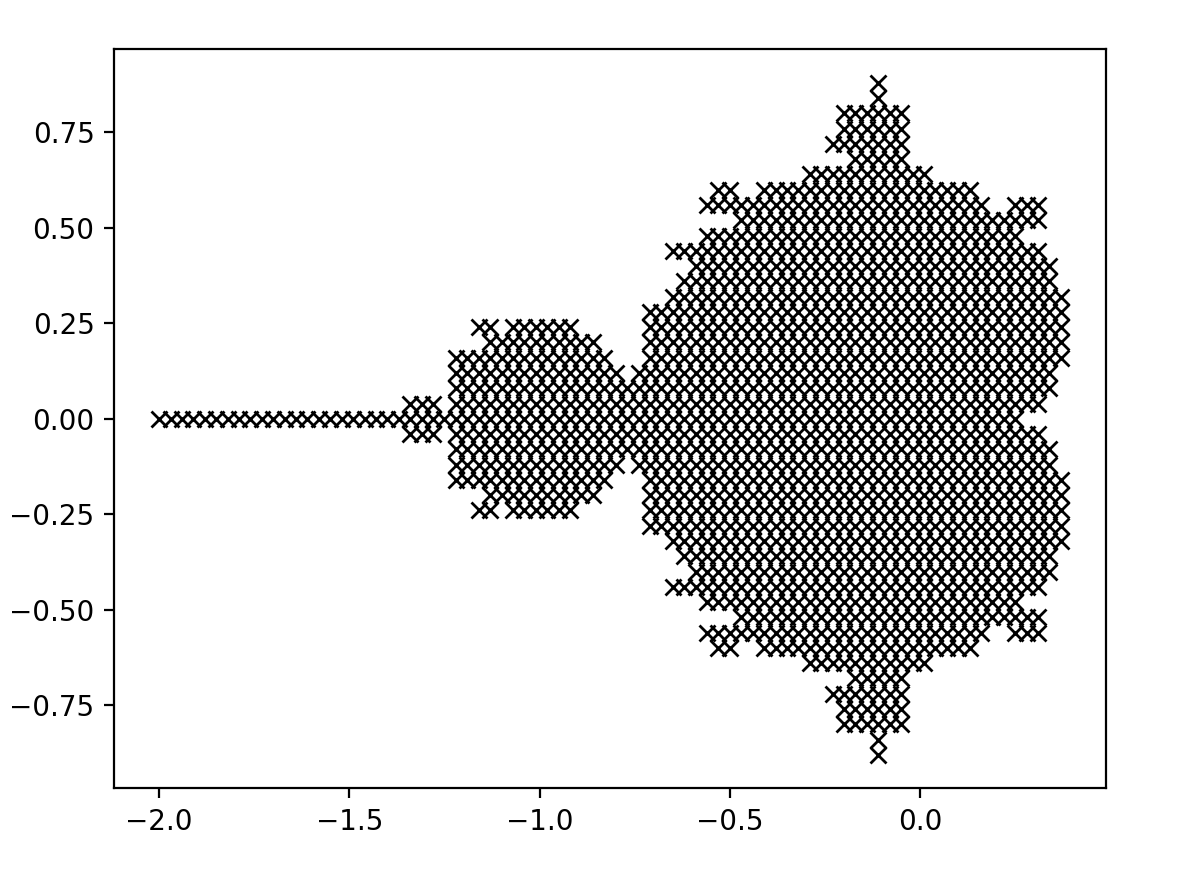
\includegraphics[scale=0.4]{mandelbrot.png}
\end{center}

\end{exercice}


\begin{correction}
\begin{enumerate}
\item Pour $c=0$ la suite $\suite{z}$ est constante égale à $0$. $0$ appartient donc à l'ensemble de Mandelbrot. 
\item Pour $c=i$, $z_0=0$, $z_1=i$, $z_2= i^2+i=-1+i$, $z_3= (-1+i)^2 +i = -i$, $z_4=(-i)^2+i = -1+i$. La suite semble périodique et donc le module est borné. Ainsi $c=i$  appartient donc à l'ensemble de Mandelbrot. 

\item Pour $c=1+i$ : $z_0=0$, $z_1=1+i$, $z_2=(1+i)^2+1+i=1+3i$, $z_3= (1+3i)^2 +1+i = -7+7i$, $z_4=(-7+7i)^2+1+i= 49(-1+i)^2+1+i = 49(-2i) +1+i = 1-97i$. Le module semble tendre vers l'infini. 
$c=1+i$ n'appartient donc pas à l'ensemble de Mandelbrot. 


\end{enumerate}
\begin{lstlisting}[language=Python]
def suite_z(n,c):
    z=0
    for i  in range(n):
        z=z**2+c
    return(z)

def verif(c):
    for n in range(101):
        if suite_z(n,c)>2:
            return(False)
    return(True)

import matplotlib.pyplot as plt
def tracer(x,y):
    c=x+y*1j
    if verif(c)==True:
        plt.plot(x,y,'kx')

for x in range(-100,101):
    for y in range(-100,101):
        tracer(x/100,y/100)
plt.show()

\end{lstlisting}

\end{correction}